\documentclass[a4paper,12pt]{article}
\usepackage[utf8]{inputenc}
\usepackage[T1]{fontenc}
\usepackage[spanish]{babel}
\usepackage{csquotes}
\usepackage{anysize}
\usepackage{graphicx}
\usepackage{hyperref}
\usepackage{pgfplots}
\pgfplotsset{compat=1.18}
%\usepackage{amsfonts}
%\usepackage{tikz}
%\usepackage{amsmath}
\marginsize{25mm}{25mm}{25mm}{25mm}

\title{Estadística inferencial}
\author{Daniel Maldonado}
\date{}

\begin{document}
{\scshape\bfseries \maketitle}

La estadística inferencial permite generalizar los resultados de muestras hacia poblaciones con niveles razonables de confianza. Esto se realiza mediante pruebas de hipótesis.

Una hipótesis experimental podría ser que la media $\bar{X}$ del grupo al cual se aplicó una intervención es distinta de la media $\mu$ de la población de la cual se obtuvo la muestra. Es decir,
\begin{eqnarray*}
    \bar{X} &<& \mu\\
            &\mbox{o}&\\
    \bar{X} &>& \mu,
\end{eqnarray*}
o de forma más general:
\[
    \bar{X} \neq \mu
.\]

Suponemos que la muestra tenía originalmente la misma media que la población, y que la aplicación de nuestra intervención desplazó su media en una cierta dirección. En cierto modo, suponemos que nuestra intervención tiene el efecto de crear una segunda población con una media distinta de la población original.

Si la muestra fuese perfectamente representativa de la población original, entonces se podría concluir que, si la media muestral $\bar{X}$ después del tratamiento es distinta de la media de la población $\mu$, entonces el tratamiento es eficaz. Sin embargo, la realidad no suele ser tan bella.

Una amenaza seria a la validez de la relación encontrada entre la aplicación del tratamiento experimental y el cambio en la media de la muestra es la posibilidad de un error de muestreo, es decir, que por azar la media de la muestra no fuese representativa de la población desde el comienzo. Esto tiene base en el {\slshape teorema central del límite} o {\slshape teorema del límite central}.

De acuerdo con el teorema podemos obtener muestras de una población y calcular la media de cada una de esas muestras. Si la cantidad de medias es lo bastante grande, entonces la distribución de esas medias tenderá a ser normal (una campana de Gauss) y la media formada por estas medias muestrales será muy cercana a la media $\mu$ de la población. Sin embargo, aunque las medias de las muestras tenderán a rondar el valor de la media poblacional, habrá una minoría que se encuentre muy lejos, ya sea por encima o por debajo. Así, existe una probabilidad nada despreciable de que la media de la muestra obtenida de la población esté muy por encima o muy por debajo del valor poblacional (Figura 1).

\begin{figure}[!ht]
  \begin{center}
    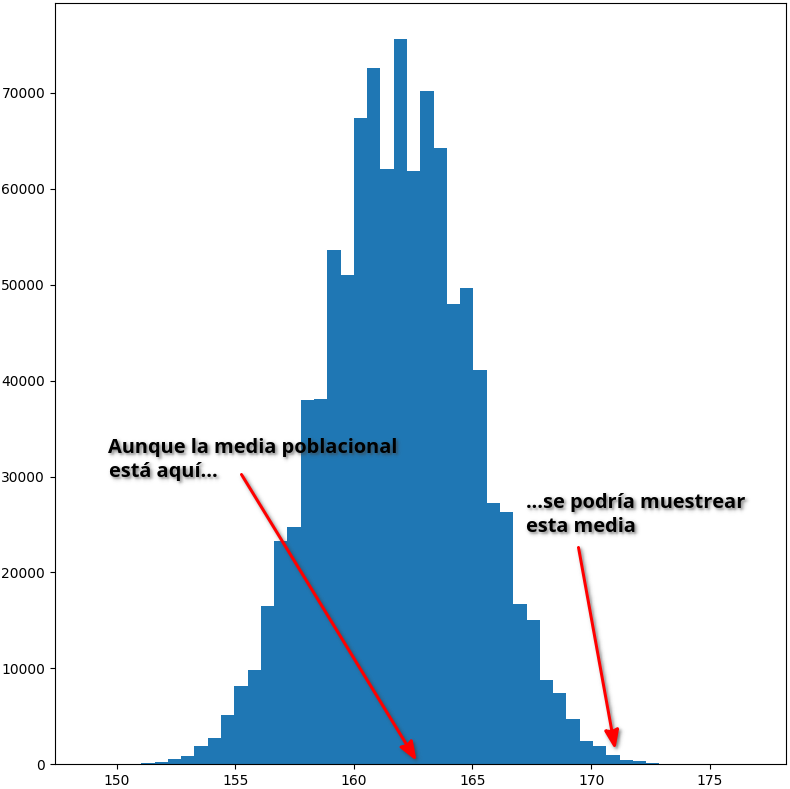
\includegraphics[scale=0.5]{curvaNormal.png}
    \caption{La media de la muestra puede estar en cualquier punto de la distribución.}
  \end{center}
\end{figure}

Si este fuera el caso, entonces la diferencia que encontramos entre la media $\bar{X}$ de la muestra tras el tratamiento y la media de la población $\mu$ sería solo debida al azar.

El papel de la estadística inferencial es garantizar que no cometamos el error de atribuir a la variable independiente (el tratamiento) las diferencias debidas a un error de muestreo. ¿Concluimos que la relación encontrada en la muestra se cumpliría si evlauamos a toda la población, o concluimos que es una coincidencia debida al error?

El procedimiento estadístico específico a usar dependerá del diseño experimental y la hipótesis, pero de modo general se puede utilizar estadística {\itshape paramétrica} y {\itshape no paramétrica}.

La estadística paramétrica requiere que se cumplan ciertos supuestos dentro de los datos de la muestra:
\begin{itemize}
  \item La población de puntuaciones de la variable dependiente forma una distribución normal (o aproximadamente normal)
  \item Las puntuaciones tienen nivel de medición de intervalos o de razón
\end{itemize}

La estadística paramétrica suele ser preferible, así que se utiliza a menos que haya flagrantes violaciones de los supuestos que tiene.

De forma general los pasos para las pruebas de hipótesis son
\begin{enumerate}
  \item Establecer una hipótesis experimental
  \item Diseñar y correr un experimento que permita probarla
  \item Traducir la hipótesis experimental en una hipótesis estadística
  \item Seleccionar y llevar a cabo el procedimiento estadístico correcto para probarla
\end{enumerate}

Las hipótesis generalmente dirán cosas similares a ``{\slshape a incrementos en X corresponden incrementos en Y}'', o ``{\slshape a incrementos en X corresponden disminuciones en Y}'', es decir, habrá una relación ordenada entre las variables, y esa relación tendrá una dirección positiva o negativa.

Si la relación es positiva, esto significará que esperamos que la media de la muestra después del tratamiento esté a la {\slshape derecha} de la media poblacional. Si la hipótesis es correcta entonces esta media muestral caerá en un punto lo bastante alejado de la media poblacional para poder decir con razonables niveles de confianza que no pertenece a la misma distribución, sino que pertenece a una nueva distribución creada por la intervención.

El punto de corte estándar en psicología es el percentil 95 de la distribución poblacional. Es decir, si la media de la muestra cae en la cola derecha de la distribución poblacional en un punto tan alejado de la media que menos del 5\% de las ocasiones en que se muestree esa distribución aparecerá un valor así de elevado, entonces tendremos suficiente certeza de que la intervención es eficaz y efectivamente desplaza los puntajes hacia la derecha.

Si anticipamos una relación negativa, ocurre lo mismo pero hacia el lado izquierdo de la distribución. Si anticipamos que habrá un cambio, pero no sabemos en qué dirección, entonces el punto de corte de 5\% se repartirá entre las dos colas de la distribución, 2.5\% de cada lado. Esta es la diferencia entre pruebas de ``una cola'' y de ``dos colas''.

\pgfmathdeclarefunction{gauss}{2}{%
  \pgfmathparse{1/(#2*sqrt(2*pi))*exp(-((x-#1)^2)/(2*#2^2))}%
}

\begin{tikzpicture}
  \begin{axis}[
    no markers, domain=-5:5, samples=100,
    axis lines*=left, xlabel=$x$, ylabel=$\bar{X}$,
    every axis y label/.style={at=(current axis.above origin),anchor=south},
    every axis x label/.style={at=(current axis.right of origin),anchor=west},
    height=5cm, width=12cm,
    xtick={0}, ytick=\empty,
    enlargelimits=false, clip=false, axis on top,
    grid = major
    ]
    \addplot [fill=cyan!20, draw=none, domain=2.5:4] {gauss(0,1)} \closedcycle;
    \addplot [fill=cyan!20, draw=none, domain=-2.5:-4] {gauss(0,1)} \closedcycle;
    \addplot [very thick,cyan!50!black] {gauss(0,1)};
    \draw (axis cs:2.5,-0.1) node [fill=white] {$5\%$} -- (axis cs: 2.5, 0.02);
    \draw (axis cs:2.8,0.1) node [fill=white] {$2{.}5\%$} -- (axis cs: 2.8, 0);
    \draw (axis cs:-2.5,-0.1) node [fill=white] {$-5\%$} -- (axis cs: -2.5, 0.02);
    \draw (axis cs:-2.8,0.1) node [fill=white] {$-2{.}5\%$} -- (axis cs: -2.8, 0);
  \end{axis}
\end{tikzpicture}

El experimento más simple es uno de una sola muestra en el cual comparamos la media de la muestra tras el tratamiento con la media de la población de origen.
La idea detrás de este diseño es comparar dos niveles de la variable independiente: el nivel experimental con otro nivel ya conocido. Un nivel conocido suele ser el de la ausencia de manipulación. Por ejemplo, si se conoce la calificación media de una población de primaria y se quiere probar una intervención que busca incrementarla entonces se tienen ya los dos niveles de la variable independiente: presencia y ausencia.

{\noindent\bfseries Ejemplo}

Una población tiene una media de puntos de IQ de 100 y una desviación estándar de 15. Queremos probar la eficacia de un tratamiento que pretende incrementar la inteligencia media.

Tomamos una muestra aleatoria de la población con tamaño de 36, le aplicamos el tratamiento, y después hacemos una medición de su IQ. El resultado es de
\[
  \bar{X} = 105
.\]
Concluimos entonces que, dado que la media de la muestra es más grande que la media de la población, el tratamiento funciona.

Fin.

\newpage

Excepto que no funciona así. Puede haber implícito un error de muestreo, y el supuesto efecto del tratamiento podría deberse al azar. Para demostrar que verdaderamente existe un efecto es necesario determinar qué tan probable es encontrar un dato tan grande como 105 o mayor en una población con  media de 100. Si la probabilidad de encontrar un dato así de grande por azar es menor al 5\%, entonces podremos concluir con relativa certeza que el cambio se debió a la intervención y no al azar (aunque nunca tendremos total seguridad de ello, porque para estar totalmente seguros deberíamos aplicar el tratamiento a la población completa y el presupuesto no alcanza para tanto).

Específicamente debemos comparar una  hipótesis nula $H_{0}$ en la cual la media de la nueva población (la población creada por nuestra intervención) es igual a la media de la población original, con una hipótesis alternativa $H_{a}$ en la cual la media de la nueva población es {\slshape distinta} de la media de la población original:
\begin{eqnarray*}
  H_{0}: & \mu = 100\\
  H_{a}: & \mu \neq 100
\end{eqnarray*}

La hipótesis nula $H_{0}$ siempre corresponderá a la ausencia de efecto o de relación entre la variable independiente y la dependiente. Si esta hipótesis es cierta, entonces concluiríamos que la media de nuestra muestra es una de las tantas medias que serían obtenidas de muestrear a la población original y no aplicar ninguna intervención.

Debe notarse que las hipótesis $H_{0}$ y $H_{a}$ componen todas las posibilidades. La media de la población con tratamiento $\mu$ puede ser igual a 100 o distinta de 100, y no hay más posibilidades. Lo mismo aplicará para cualquier prueba de hipótesis que realicemos: las hipótesis propuestas deben agotar el espacio de las posibilidades.

Para este caso particular el procedimiento estadístico usado se conoce como prueba {\itshape z}. Este procedimiento consiste en calcular el puntaje {\itshape z} de la media de la muestra tras el tratamiento, y después determinar la localización de esa media en la distribución de la población dada por el teorema central del límite. Recordemos que el puntaje z de un dato indica cuánto éste se desvía de la media de su población o qué tan atípico es con respecto a ella, y se calcula restándole la media y dividiendo el resultado entre la desviación estándar:
\[
z = \frac{
  X - \bar{X}
}{
  S_{X}
}
.\]

Este diseño requiere que la distribución de la variable dependiente sea aproximadamente normal y que la muestra haya sido seleccionada de forma aleatoria. Además, es indispensable conocer la media de la población y su desviación estándar, lo que por lo general no ocurrirá. Pero supongamos que sí por esta ocasión.

Para hacer la comparación entre la media muestral y la media de la población suponemos una distribución formada por infinitas medias muestrales con tamaño de 36 (porque ese es el tamaño de la muestra dado en el ejemplo). La media de esta distribución muestral estará muy cerca de la media verdadera de la población. Entonces, esta distribución muestral indicará la frecuencia de todas las $\bar{X}$ que podrían encontrarse si se toman infinitas muestras aleatorias de tamaño 36 de la población. Suponiendo que $H_{0}$ sea correcta, toda media distinta de 100 vendrá de error de muestreo de esta distribución.

El siguiente paso será determinar el umbral de aceptación que se utilizará para la comparación, es decir, cuánto riesgo de equivocarnos estamos dispuestos a aceptar. En psicología el riesgo aceptable es del 5\% por convención, pero en otras áreas (como medicina) no se acepta más del 1\%. Este umbral se denomina $\alpha$:
\[
  \alpha = 0{.}05
\]

$\alpha = 0{.}05$ indica que estamos dispuestos a aceptar un riesgo de equivocarnos del 5\% y, por lo tanto, concluir una de cada 20 veces que existe un efecto de la variable independiente cuando esto no es real (y la variación en los datos se debió a un error de muestreo).

¿Por qué no usar un $\alpha$ más estricto? Porque eso podría significar arriesgarse a ignorar un efecto real, es decir, concluir que no existe un efecto por parte de la variable independiente cuando en realidad sí lo hubo.

Estos dos tipos de errores---falso positivo y falso negativo---se conocen también como errores de tipo I y tipo II o errores $\alpha$ y $\beta$.

\begin{figure}[!ht]
  \begin{center}
    \begin{tabular}{|p{3cm}|p{3cm}|p{3cm}|}
      \hline
  &Existe Efecto&No Existe Efecto\\
  \hline
      Decimos que sí\newline existe efecto&Correcto&Falso positivo\newline Error tipo I\newline Error $\alpha$\\
      \hline
      Decimos que no existe efecto&Falso negativo\newline Error tipo II\newline Error $\beta$&Correcto\\
      \hline
    \end{tabular}
  \end{center}
\end{figure}

$\alpha$ y $\beta$ son complementarios y en conjunto deben sumar 1. Cuanto mayor sea $\alpha$, mayor la probabilidad de concluir que sí existe un efecto cuando no lo hay, pero también mayor la probabilidad de detectar efectos que sí existen. Cuanto mayor es $\beta$ mayor será la probabilidad de pasar por alto efectos reales, pero también menor será la probabilidad de concluir que sí existe un efecto cuando no lo hay.

Una vez elegido el umbral $\alpha$, éste se debe localizar dentro de la distribución de medias muestrales. El umbral estará repartido entre ambas colas de la distribución en este caso debido a que nuestra hipótesis es únicamente que el IQ medio cambiará, pero no predecimos la dirección.

La localización del umbral $\alpha$ dentro de la distribución está dada por tablas que pueden encontrarse en internet o en libros de estadística. La tabla de $z$ es sencilla debido a que indica solo la ubicación en porcentaje de un punto $z$ particular. En el caso del umbral de $0{.}025\%$ (porque al ser una prueba de dos colas dividimos $\alpha$ entre 2) la traducción en puntaje $z$ es de $\pm 1.96$. Es decir, el umbral de $\pm 2{.}5\%$ está localizado a $\pm$1.96 desviaciones estándar de la media de una distribución normal. Este valor será llamado $z_{crit}$.

Lo único que resta es convertir el valor de la media de la muestra, 105, en puntaje $z$ y compararlo con $z_{crit}$. La fórmula para computar el puntaje $z$ de los datos ($z_{obt}$) es:
\[
z_{obt} = \frac{
  \bar{X} - \mu
}{
  \sigma_{\bar{X}}
}
\]
donde
\[
  \sigma_{\bar{X}} = \frac{
    \sigma_{X}
  }{
    \sqrt{N}
  }
\]
Es decir, se obtiene la diferencia entre la media muestral y la poblacional ($\bar{X} - \mu$), y se divide entre el error estándar de la media ($\sigma_{\bar{X}}$).

Calculamos primero el error estándar de la media. N es el tamaño de la muestra, y $\sigma_{X}$ es la desviación estándar de la población. Para el ejemplo con $\sigma_X = 5$ y $N = 36$:
\[
  \sigma_{\bar{X}} = \frac{
    \sigma_{X}
  }{
    \sqrt{N}
  } = \frac{
    15
  }{
    \sqrt{36}
  } = \frac{
    15
  }{
    6
  } = 2{.}5
\]
Después computamos $z_{obt}$. $\mu$ será la media de la población, $\bar{X}$ se obtiene de la muestra, y $\sigma_{\bar{X}}$ es el error estándar que acabamos de calcular. Entonces:
\[
z_{obt} = \frac{
  \bar{X} - \mu
}{
  \sigma_{\bar{X}}
} = \frac{
  105 - 100
}{
  2{.}5
} = \frac{
  +5
}{
  2{.}5
} = +2{.}00
\]
Nuestro $z_{obt}$ es +2.00. Para interpretar lo que esto significa es necesario compararlo con $z_{crit}$.

El valor de $z_{crit}$ era de $\pm 1{.}96$. Dado que el valor de +2.00 es más grande sabemos que la media de nuestra muestra se encuentra más allá del umbral de $\alpha = 0{.}025$:

\begin{tikzpicture}
  \begin{axis}[
    no markers, domain=-5:5, samples=100,
    axis lines*=left, xlabel=$x$, ylabel=$\bar{X}$,
    every axis y label/.style={at=(current axis.above origin),anchor=south},
    every axis x label/.style={at=(current axis.right of origin),anchor=west},
    height=5cm, width=12cm,
    xtick={0}, ytick=\empty,
    enlargelimits=false, clip=false, axis on top,
    grid = major
    ]
    \addplot [fill=cyan!20, draw=none, domain=2.5:4] {gauss(0,1)} \closedcycle;
    \addplot [fill=cyan!20, draw=none, domain=-2.5:-4] {gauss(0,1)} \closedcycle;
    \addplot [very thick,cyan!50!black] {gauss(0,1)};
    \draw (axis cs:2.7,-0.1) node [fill=white] {$z_{crit} = 1{.}96$} -- (axis cs: 2.7, 0.02);
    \draw (axis cs:2.8,0.1) node [fill=white] {$z_{obt} = 2{.}00$} -- (axis cs: 2.8, 0);
  \end{axis}
\end{tikzpicture}

Esto indica que podemos {\slshape rechazar} la hipótesis nula $H_{0}$ a favor de la hipótesis alternativa $H_{a}$, es decir, que podemos concluir con un nivel razonable de confianza que nuestra muestra con media de $\bar{X} = 105$ difícilmente podría haber venido de una población con una media de $\mu = 100$, y que lo más probable es que venga de una población distinta, probablemente la población ``creada'' por nuestra intervención.

Dicho de otra forma, decimos que nuestros resultados son {\slshape significativos}. Significativo no quiere decir {\slshape importante}, solo que difícilmente ocurrirían si no existiese una relación en la población. Es importante notar que tampoco hemos demostrado que nuestra intervención funciona, sino solamente que una muestra como la que encontramos sería improbable si la intervención no funcionase, pero esto aun es una posibilidad. Y tampoco demostramos que es nuestra variable independiente lo que ocasionó el cambio. Esto aun pudo deberse a factores fuera de nuestro control experimental. Por ello es importante replicar los estudios en ciencia.


\end{document}
